\documentclass[main]{subfiles}
\begin{document}

%@@@@@@@@@@@@@@@@@@@@@@@@@@@@@@
% Main Topics: Digital logic, Linear Threshold Unit/Gates 29.11.2018
% Lecturer: Matthew Cook
% author: Vanessa Leite - base document from benelot/eth-intro-to-neuroinformatics-summary

\section{Digital Logic}

We don't learn how the brain works by studying neurons, the same way that just by studying transistors we do not know how computer works.
We know the brain does processing but we don't know how it works. The bottleneck to understand brain is probably that we do not have the right abstractions to understand it.

\subsection{(Basic) Digital Logic}

Gates are processing units.

\begin{figure}[H]
	\centering
	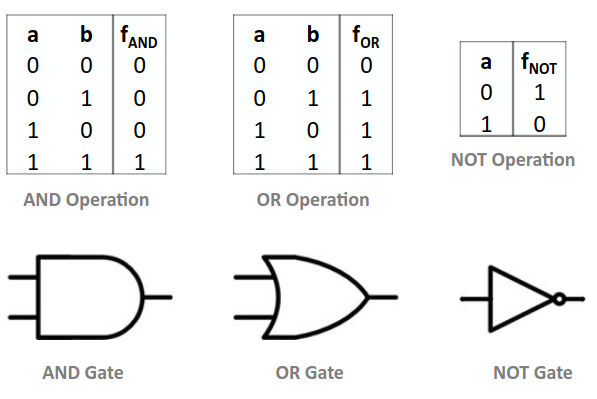
\includegraphics[width=0.5\textwidth]{basic-gates.png}
\end{figure}

Circuits are a combination of gates.

\begin{figure}[H]
	\centering
	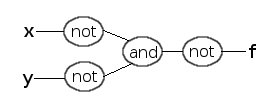
\includegraphics[width=0.4\textwidth]{circuit.png}
	\label{fig:circuit}
	\caption{A basic circuit implementing an OR gate.}
\end{figure}

The circuit in Fig~\ref{fig:circuit} produces the same as an OR gate. With NOT and AND gates we can build an OR gate, but with AND and OR we can't build a NOT gate.

\paragraph{XOR gates = exclusive OR}
They are exclusive in the case of two inputs. For more than two, XOR counts the number of "active" ($1$'s) inputs and returns $0$ for even and $1$ for odd.

\begin{figure}[H]
	\centering
	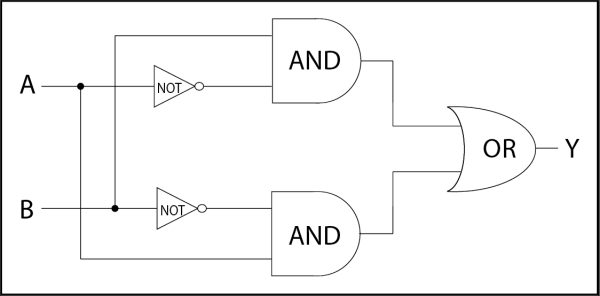
\includegraphics[width=0.5\textwidth]{gatexor.png}
	\caption{XOR gate built out other gates. Image from https://blog.digilentinc.com/building-logic-gates-with-transistors/}
\end{figure}

A table with $N$ inputs has $2^N$ rows.

\paragraph{Other gates}

\begin{tabular}{|c|c|c|c|c|c|c|c|c|}
	\hline
	\multicolumn{2}{|c|}{Input} &
	\multicolumn{7}{|c|}{Output}\\\hline
	A & B & AND & OR & NOT & XOR & NAND & NOR & XNOR\\\hline
	  &   & \scalebox{0.4}{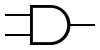
\includegraphics{100px-AND_ANSI.png}} & \scalebox{0.4}{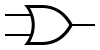
\includegraphics{100px-OR_ANSI.png}} &\scalebox{0.4}{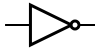
\includegraphics{100px-NOT_ANSI.png}} &\scalebox{0.4}{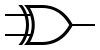
\includegraphics{100px-XOR_ANSI.png}} &\scalebox{0.4}{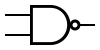
\includegraphics{100px-NAND_ANSI.png}} &\scalebox{0.4}{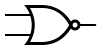
\includegraphics{100px-NOR_ANSI.png}} &\scalebox{0.4}{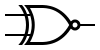
\includegraphics{100px-XNOR_ANSI.png}}\\\hline
	0 & 0 & 0 & 0 & 1 & 0 & 1 & 1 & 1\\\hline
	0 & 1 & 0 & 1 & 1 & 1 & 1 & 0 & 0\\\hline
	1 & 0 & 0 & 1 & 0 & 1 & 1 & 0 & 0\\\hline
	1 & 1 & 1 & 1 & 0 & 0 & 0 & 0 & 1\\\hline
\end{tabular}

\subsection{Linear Threshold (LT) Unit/Gates (Perceptron)}

\begin{figure}[H]
	\centering
	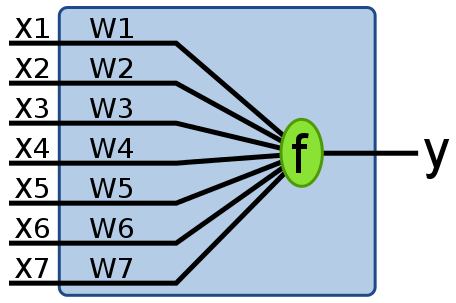
\includegraphics[width=0.3\textwidth]{perceptron.png}
\end{figure}

This model represents a neuron with inputs $x$ and one output $y$. Weights $w$ determine the influence of the inputs. $f$ is a function determining the output: if the influence of all the inputs combined cross a threshold, then the neuron become active. Active state: $\sum_i(w_i\cdot x_i) \geq \theta$. Otherwise, the neuron is inactive.

We add a bias input as $-\theta$ so that $w_0+\sum_i(w_i\cdot x_i)\geq0$ activates the neuron.

This model can create AND/OR/NOT-Gates. Not the XOR/XNOR-Gate however.

\subsubsection{XOR impossibility with LT/Perceptrons}
To compute XOR with LT, it is required that:

\begin{itemize}[noitemsep,nolistsep]
	\item $w_0 < 0$
	\item $x_2 \times w_2 + w_0 \geq 0$
	\item $x_1 \times w_1 + w_0 \geq 0$
	\item $x_1 \times w_1 + x_2 \times w_2 + w_0 < 0$.
\end{itemize}

This causes a contradiction because $x_1 \times w_1 + x_2 \times w_2 + 2 \times w_0 < 0$ and $x_1 \times w_1 + x_2 \times w_2 + 2 \times w_0 \geq 0$ when adding up the constraints.

XOR is not a linear combination of the inputs.

\subsection{McCulloch-Pitts Neuron / Perceptron}
\textbf{Similarities to real neurons:}
\begin{itemize}[noitemsep,nolistsep]
	\item Both can be active or inactive.
	\item The input/output is directed.
	\item The activation of a neuron is dependent on a weighted function of other neurons.
\end{itemize}
\textbf{Differences to real neurons:}
\begin{itemize}[noitemsep,nolistsep]
	\item Real neurons exist in continuous time, whereas McCulloch-Pitts neurons operate in discrete time.
	\item Real neurons have degrees of activation, not just on/off.
	\item The activation as a function of the inputs of real neuron is typically not linear or threshold linear.
\end{itemize}

\end{document}
